\documentclass{article}
\setlength{\parindent}{0pt}
\setlength{\parskip}{2ex plus 0.5ex minus 0.2ex}
\usepackage[margin=1in]{geometry}
\renewcommand{\topfraction}{0.9}
\renewcommand{\bottomfraction}{0.8}
\setcounter{topnumber}{2}
\setcounter{bottomnumber}{2}
\setcounter{totalnumber}{4}
\renewcommand{\textfraction}{0.07}
\renewcommand{\floatpagefraction}{0.7}
\usepackage{graphicx}
\usepackage{textcomp}
\usepackage{placeins}
\usepackage[T1]{fontenc}
\usepackage{gensymb}
\usepackage[utf8]{inputenc}
\usepackage{caption}
\usepackage[export]{adjustbox}
\graphicspath{{./figures/}}
% hyperref usually has to go last
\usepackage[hidelinks]{hyperref}
% but glossaries behaves best if after hyperref
\usepackage[acronym,toc]{glossaries}
%\newacronym{<++>}{<++>}{<++>}
\newacronym[longplural={metric tons of heavy metal}]{MTHM}{MTHM}{metric ton of heavy metal}
\newacronym{ABM}{ABM}{agent-based modeling}
\newacronym{ACDIS}{ACDIS}{Program in Arms Control \& Domestic and International Security}
\newacronym{AHTR}{AHTR}{Advanced High Temperature Reactor}
\newacronym{ANDRA}{ANDRA}{Agence Nationale pour la gestion des D\'echets RAdioactifs, the French National Agency for Radioactive Waste Management}
\newacronym{ANL}{ANL}{Argonne National Laboratory}
\newacronym{ANS}{ANS}{American Nuclear Society}
\newacronym{API}{API}{application programming interface}
\newacronym{ARE}{ARE}{Aircraft Reactor Experiment}
\newacronym{ARFC}{ARFC}{Advanced Reactors and Fuel Cycles}
\newacronym{ASME}{ASME}{American Society of Mechanical Engineers}
\newacronym{ATWS}{ATWS}{Anticipated Transient Without Scram}
\newacronym{BDBE}{BDBE}{Beyond Design Basis Event}
\newacronym{BIDS}{BIDS}{Berkeley Institute for Data Science}
\newacronym{CAFCA}{CAFCA}{ Code for Advanced Fuel Cycles Assessment }
\newacronym{CDTN}{CDTN}{Centro de Desenvolvimento da Tecnologia Nuclear}
\newacronym{CEA}{CEA}{Commissariat \`a l'\'Energie Atomique et aux \'Energies Alternatives}
\newacronym{CI}{CI}{continuous integration}
\newacronym{CNEN}{CNEN}{Comiss\~{a}o Nacional de Energia Nuclear}
\newacronym{CNERG}{CNERG}{Computational Nuclear Engineering Research Group}
\newacronym{COSI}{COSI}{Commelini-Sicard}
\newacronym{COTS}{COTS}{commercial, off-the-shelf}
\newacronym{CSNF}{CSNF}{commercial spent nuclear fuel}
\newacronym{CTAH}{CTAHs}{Coiled Tube Air Heaters}
\newacronym{CUBIT}{CUBIT}{CUBIT Geometry and Mesh Generation Toolkit}
\newacronym{CURIE}{CURIE}{Centralized Used Fuel Resource for Information Exchange}
\newacronym{DAG}{DAG}{directed acyclic graph}
\newacronym{DANESS}{DANESS}{Dynamic Analysis of Nuclear Energy System Strategies}
\newacronym{DBE}{DBE}{Design Basis Event}
\newacronym{DESAE}{DESAE}{Dynamic Analysis of Nuclear Energy Systems Strategies}
\newacronym{DHS}{DHS}{Department of Homeland Security}
\newacronym{DOE}{DOE}{Department of Energy}
\newacronym{DRACS}{DRACS}{Direct Reactor Auxiliary Cooling System}
\newacronym{DRE}{DRE}{dynamic resource exchange}
\newacronym{DSNF}{DSNF}{DOE spent nuclear fuel}
\newacronym{DYMOND}{DYMOND}{Dynamic Model of Nuclear Development }
\newacronym{EBS}{EBS}{Engineered Barrier System}
\newacronym{EDF}{EDF}{Électricité de France}
\newacronym{EDZ}{EDZ}{Excavation Disturbed Zone}
\newacronym{EIA}{EIA}{U.S. Energy Information Administration}
\newacronym{EPA}{EPA}{Environmental Protection Agency}
\newacronym{EPR}{EPR}{European Pressurized Reactors}
\newacronym{EP}{EP}{Engineering Physics}
\newacronym{EU}{EU}{European Union}
\newacronym{FCO}{FCO}{Fuel Cycle Options}
\newacronym{FCT}{FCT}{Fuel Cycle Technology}
\newacronym{FEHM}{FEHM}{Finite Element Heat and Mass Transfer}
\newacronym{FEPs}{FEPs}{Features, Events, and Processes}
\newacronym{FHR}{FHR}{Fluoride-Salt-Cooled High-Temperature Reactor}
\newacronym{FLiBe}{FLiBe}{Fluoride-Lithium-Beryllium}
\newacronym{FP}{FP}{Fission Products}
\newacronym{GDSE}{GDSE}{Generic Disposal System Environment}
\newacronym{GDSM}{GDSM}{Generic Disposal System Model}
\newacronym{GENIUSv1}{GENIUSv1}{Global Evaluation of Nuclear Infrastructure Utilization Scenarios, Version 1}
\newacronym{GENIUSv2}{GENIUSv2}{Global Evaluation of Nuclear Infrastructure Utilization Scenarios, Version 2}
\newacronym{GENIUS}{GENIUS}{Global Evaluation of Nuclear Infrastructure Utilization Scenarios}
\newacronym{GPAM}{GPAM}{Generic Performance Assessment Model}
\newacronym{GRSAC}{GRSAC}{Graphite Reactor Severe Accident Code}
\newacronym{GUI}{GUI}{graphical user interface}
\newacronym{HLW}{HLW}{high level waste}
\newacronym{HPC}{HPC}{high-performance computing}
\newacronym{HTC}{HTC}{high-throughput computing}
\newacronym{HTGR}{HTGR}{High Temperature Gas-Cooled Reactor}
\newacronym{IAEA}{IAEA}{International Atomic Energy Agency}
\newacronym{IEMA}{IEMA}{Illinois Emergency Mangament Agency}
\newacronym{IHLRWM}{IHLRWM}{International High Level Radioactive Waste Management}
\newacronym{INL}{INL}{Idaho National Laboratory}
\newacronym{IPRR1}{IRP-R1}{Instituto de Pesquisas Radioativas Reator 1}
\newacronym{IRP}{IRP}{Integrated Research Project}
\newacronym{ISFSI}{ISFSI}{Independent Spent Fuel Storage Installation}
\newacronym{ISRG}{ISRG}{Independent Student Research Group}
\newacronym{JFNK}{JFNK}{Jacobian-Free Newton Krylov}
\newacronym{LANL}{LANL}{Los Alamos National Laboratory}
\newacronym{LBNL}{LBNL}{Lawrence Berkeley National Laboratory}
\newacronym{LCOE}{LCOE}{levelized cost of electricity}
\newacronym{LDRD}{LDRD}{laboratory directed research and development}
\newacronym{LFR}{LFR}{Lead-Cooled Fast Reactor}
\newacronym{LLNL}{LLNL}{Lawrence Livermore National Laboratory}
\newacronym{LMFBR}{LMFBR}{Liquid Metal Fast Breeder Reactor}
\newacronym{LOFC}{LOFC}{Loss of Forced Cooling}
\newacronym{LOHS}{LOHS}{Loss of Heat Sink}
\newacronym{LOLA}{LOLA}{Loss of Large Area}
\newacronym{LP}{LP}{linear program}
\newacronym{LWR}{LWR}{Light Water Reactor}
\newacronym{MAGNOX}{MAGNOX}{Magnesium Alloy Graphie Moderated Gas Cooled Uranium Oxide Reactor}
\newacronym{MA}{MA}{minor actinide}
\newacronym{MCNP}{MCNP}{Monte Carlo N-Particle code}
\newacronym{MILP}{MILP}{mixed-integer linear program}
\newacronym{MIT}{MIT}{the Massachusetts Institute of Technology}
\newacronym{MOAB}{MOAB}{Mesh-Oriented datABase}
\newacronym{MOOSE}{MOOSE}{Multiphysics Object-Oriented Simulation Environment}
\newacronym{MOX}{MOX}{mixed oxide}
\newacronym{MSBR}{MSBR}{Molten Salt Breeder Reactor}
\newacronym{MSRE}{MSRE}{Molten Salt Reactor Experiment}
\newacronym{MSR}{MSR}{Molten Salt Reactor}
\newacronym{NAGRA}{NAGRA}{National Cooperative for the Disposal of Radioactive Waste}
\newacronym{NEAMS}{NEAMS}{Nuclear Engineering Advanced Modeling and Simulation}
\newacronym{NEUP}{NEUP}{Nuclear Energy University Programs}
\newacronym{NFCSim}{NFCSim}{Nuclear Fuel Cycle Simulator}
\newacronym{NGNP}{NGNP}{Next Generation Nuclear Plant}
\newacronym{NMWPC}{NMWPC}{Nuclear MW Per Capita}
\newacronym{NNSA}{NNSA}{National Nuclear Security Administration}
\newacronym{NPP}{NPP}{Nuclear Power Plant}
\newacronym{NPRE}{NPRE}{Department of Nuclear, Plasma, and Radiological Engineering}
\newacronym{NQA1}{NQA-1}{Nuclear Quality Assurance - 1}
\newacronym{NRC}{NRC}{Nuclear Regulatory Commission}
\newacronym{NSF}{NSF}{National Science Foundation}
\newacronym{NSSC}{NSSC}{Nuclear Science and Security Consortium}
\newacronym{NUWASTE}{NUWASTE}{Nuclear Waste Assessment System for Technical Evaluation}
\newacronym{NWF}{NWF}{Nuclear Waste Fund}
\newacronym{NWTRB}{NWTRB}{Nuclear Waste Technical Review Board}
\newacronym{OCRWM}{OCRWM}{Office of Civilian Radioactive Waste Management}
\newacronym{ORION}{ORION}{ORION}
\newacronym{ORNL}{ORNL}{Oak Ridge National Laboratory}
\newacronym{PARCS}{PARCS}{Purdue Advanced Reactor Core Simulator}
\newacronym{PBAHTR}{PB-AHTR}{Pebble Bed Advanced High Temperature Reactor}
\newacronym{PBFHR}{PB-FHR}{Pebble-Bed Fluoride-Salt-Cooled High-Temperature Reactor}
\newacronym{PEI}{PEI}{Peak Environmental Impact}
\newacronym{PH}{PRONGHORN}{PRONGHORN}
\newacronym{PRIS}{PRIS}{Power Reactor Information System}
\newacronym{PRKE}{PRKE}{Point Reactor Kinetics Equations}
\newacronym{PSPG}{PSPG}{Pressure-Stabilizing/Petrov-Galerkin}
\newacronym{PWAR}{PWAR}{Pratt and Whitney Aircraft Reactor}
\newacronym{PWR}{PWR}{Pressurized Water Reactor}
\newacronym{PyNE}{PyNE}{Python toolkit for Nuclear Engineering}
\newacronym{PyRK}{PyRK}{Python for Reactor Kinetics}
\newacronym{QA}{QA}{quality assurance}
\newacronym{RDD}{RD\&D}{Research Development and Demonstration}
\newacronym{RD}{R\&D}{Research and Development}
\newacronym{RELAP}{RELAP}{Reactor Excursion and Leak Analysis Program}
\newacronym{RIA}{RIA}{Reactivity Insertion Accident}
\newacronym{RIF}{RIF}{Region-Institution-Facility}
\newacronym{SFR}{SFR}{Sodium-Cooled Fast Reactor}
\newacronym{SINDAG}{SINDA{\textbackslash}G}{Systems Improved Numerical Differencing Analyzer $\backslash$ Gaski}
\newacronym{SKB}{SKB}{Svensk K\"{a}rnbr\"{a}nslehantering AB}
\newacronym{SNF}{SNF}{spent nuclear fuel}
\newacronym{SNL}{SNL}{Sandia National Laboratory}
\newacronym{STC}{STC}{specific temperature change}
\newacronym{SUPG}{SUPG}{Streamline-Upwind/Petrov-Galerkin}
\newacronym{SWF}{SWF}{Separations and Waste Forms}
\newacronym{SWU}{SWU}{Separative Work Unit}
\newacronym{TRIGA}{TRIGA}{Training Research Isotope General Atomic}
\newacronym{TRISO}{TRISO}{Tristructural Isotropic}
\newacronym{TSM}{TSM}{Total System Model}
\newacronym{TSPA}{TSPA}{Total System Performance Assessment for the Yucca Mountain License Application}
\newacronym{ThOX}{ThOX}{thorium oxide}
\newacronym{UFD}{UFD}{Used Fuel Disposition}
\newacronym{UML}{UML}{Unified Modeling Language}
\newacronym{UOX}{UOX}{uranium oxide}
\newacronym{UQ}{UQ}{uncertainty quantification}
\newacronym{US}{US}{United States}
\newacronym{UW}{UW}{University of Wisconsin}
\newacronym{VISION}{VISION}{the Verifiable Fuel Cycle Simulation Model}
\newacronym{VVER}{VVER}{Voda-Vodyanoi Energetichesky Reaktor (Russian Pressurized Water Reactor)}
\newacronym{VV}{V\&V}{verification and validation}
\newacronym{WIPP}{WIPP}{Waste Isolation Pilot Plant}
\newacronym{YMR}{YMR}{Yucca Mountain Repository Site}

\makeglossaries
% cleveref only behaves if after hyperref & glossaries
\usepackage{cleveref}
\usepackage{minted}
\usepackage{ifthen}
\usepackage{subcaption}
%% \usepackage{listings}  % Allows code printing
%% \definecolor{codegreen}{rgb}{0,0.6,0}
%% \definecolor{codegray}{rgb}{0.5,0.5,0.5}
%% \definecolor{codepurple}{rgb}{0.58,0,0.82}
%% \definecolor{backcolour}{rgb}{0.95,0.95,0.92}
%% \lstdefinestyle{mystyle}{
%%     backgroundcolor=\color{backcolour},
%%     commentstyle=\color{codegreen},
%%     keywordstyle=\color{magenta},
%%     numberstyle=\tiny\color{codegray},
%%     stringstyle=\color{codepurple},
%%     basicstyle=\footnotesize,
%%     breakatwhitespace=false,
%%     breaklines=true,
%%     captionpos=b,
%%     keepspaces=true,
%%     numbers=left,
%%     numbersep=5pt,
%%     showspaces=false,
%%     showstringspaces=false,
%%     showtabs=false,
%%     tabsize=2
%% }
%% \lstset{style=mystyle}


\let\Oldsection\section
\renewcommand{\section}{\FloatBarrier\Oldsection}

\let\Oldsubsection\subsection
\renewcommand{\subsection}{\FloatBarrier\Oldsubsection}

\let\Oldsubsubsection\subsubsection
\renewcommand{\subsubsection}{\FloatBarrier\Oldsubsubsection}

\newcommand{\code}[1]{\texttt{#1}}
\makeatletter
\def\maxwidth#1{\ifdim\Gin@nat@width>#1 #1\else\Gin@nat@width\fi}
\makeatother

\title{Introduction to Moltres: an Application for Simulation of Molten Salt Reactors}
\author{Alexander Lindsay, Gavin Ridley, Kathryn Huff}

\begin{document}
\maketitle

\begin{abstract}

Moltres is a new physics application for modeling coupled physics in 
fluid-fuelled, molten salt reactors. This paper describes its neutronics model, 
thermal hydraulics model, and their coupling in the MOOSE framework. Neutron 
and precursor equations are implemented using an Action system that allows use 
of an arbitrary number of groups with no change in the input card. Results for 
many-channel configurations in 2D-axisymmetric and 3D coordinates are presented 
and compared against other coupled models as well as the Molten Salt Reactor 
Experiment.

\end{abstract}

\section{Introduction}

Molten salt reactor concepts garnered considerable interest in the 1950s and 60s
with development of the \gls{ARE} and later the \gls{MSRE} at \gls{ORNL}.  With
the inclusion of the \gls{MSR} among the Generation-IV reactor designs
\cite{gif_generation_2008,gif_generation_2015}, this reactor concept has gained renewed research
interest in the past decade, with many new nuclear companies proposing both
fluid-fuelled and solid-fuelled commercial \gls{MSR} designs
\cite{hyde_liquid_2015,leblanc_integral_2015,thorcon_-able_2017,scarlat_design_2014,transatomic_power_corporation_neutronics_2016}. 
Two key advantages offered by the fluid-fuelled \gls{MSR} are improved fuel
utilization and no radiation damage constraint on attainable fuel
burn-up. Together, these attributes result in significantly reduced core fissile
inventories and spent nuclear fuel mass 
\cite{gif_generation_2008,gif_generation_2015}.  
Due to these characteristics, the \gls{MSR} is potentially uniquely capable of 
burning actinides and extending fuel resources.

Simulation tools developed by many authors successfully describe steady-state and
transient behavior of myriad \gls{MSR} concepts. Krepel et al. extended the in-house \gls{LWR}
diffusion code DYN3D to consider drift of delayed neutron precursors alongside
the reactor temperature profile, re-casting the extended code as
DYN3D-MSR \cite{krepel_dyn3d-msr_2007}. That work compared DYN3D-MSR against
experimental \gls{MSRE} data and then used it to simulate local fuel channel
blockages as well as local temperature perturbations. 

In a similar vein, Kophazi et. al. used iterative coupling between in-house
three-dimensional neutronic and one-dimensional heat conduction models DALTON
and THERM to analyze normal \gls{MSRE} operation as well as
channel-blocking-incident transients \cite{kophazi_development_2009}. The
Kophazi model added entrance effects of heat transfer coefficients as well as
thermal coupling between fuel channels through moderator heat conduction. More
recently, Cammi et. al. performed a 2D-axisymmetric single-channel analysis of
the \gls{MSBR} using the commercial finite element package COMSOL Multiphysics
\cite{cammi_multi-physics_2011}. That work directly solved the fuel salt
velocity field, used heterogeneous group constants in fuel and moderator
regions, and employed the \gls{COMSOL} software package intrinsically designed
for coupled multi-physics simulation.  Fiorina, Lathouwers, and their
colleagues conducted a benchmarking exercise \cite{fiorina_modelling_2013} in
which this Politecnico di Milano approach was expanded to a multi-channel model 
of the \gls{MSFR} and compared to code from the University of Delft
\cite{de_zwaan_static_2007,van_der_linden_2012} based on the approach in
\cite{kophazi_development_2009}. These models showed good agreement for
multiple accident transients. Meanwhile, leveraging lessons learned from these 
efforts has resulted in a multiscale approach from Zanetti et al. 
\cite{zanetti_geometric_2015} successfully combines high and low geometric 
fidelity for graphite-moderated \glspl{MSR}.

More recently, Aufiero et.  al \cite{aufiero_development_2014} have begun to
approach transient simulations in the \gls{MSFR} within the finite volume
OpenFOAM multiphysics toolkit\cite{weller_tensorial_1998}.  This approach
benefits from pre-implemented turbulence models available in the OpenFOAM
library and captures the full-core three-dimensional geometry of the reactor
primary circuit.  OpenFOAM \gls{CFD} has additionally been shown by Laureau et
al. \cite{laureau_transient_2017} to couple well with Transient Fission Matrix
neutronics within the \gls{MSFR}.

The present work introduces the open source simulation tool, Moltres
\cite{lindsay_moltres_2017}, for simulating \glspl{MSR}.  By implementing
deterministic neutronics and thermal hydraulics in the context of the
\gls{MOOSE} finite element modeling framework, Moltres solves arbitrary-group
neutron diffusion, temperature, and precursor governing equations in anywhere
from one to three dimensions and can be deployed on an arbitrary number of
processing units.

Moltres is an open source code licensed under \gls{LGPL} terms so the 
\gls{MSR} community can freely use, interrogate, and improve it.  Its openness 
is a defining characteristic and promotes
quality through transparency and ease of peer review. In the era of
GitHub\cite{github_build_2017} and international scientific collaboration,
open and modern software practices must be employed in order for nuclear
engineering simulation capability to enable discovery and support the regulatory
needs presented by new reactor designs. In that vein, Moltres uses
\mintinline{latex}{git} for version control, integration testing to protect
developed physics capabilities, and a C++ object-oriented design to
enable extension and code reuse. Moreover, Moltres depends on the \gls{MOOSE} 
framework, \cite{gaston_physics-based_2015} another \gls{LGPL} code that itself 
leans on LibMesh \cite{kirk_libmesh:_2006}, a
\gls{LGPL} finite element library, and PetSc \cite{satish_balay_petsc_2015}, a
\gls{BSD}-licensed toolkit for solving nonlinear equations yielded by 
discretizing PDEs. \gls{MOOSE} and LibMesh translate weak PDE forms defined by
applications (e.g. Moltres) into residual and Jacobian
functions. These functions are the inputs into PetSc Newton-Raphson solution routines. All
codes use MPI for parallel communication and are easily deployed on
massively-parallel cluster-computing platforms. \gls{MOOSE} applications by
default use monolithic and implicit methods ideal for closely-coupled
and multi-scale physics, such as the model problem described
in this work. However, Moltres can also use explicit
time-stepping routines as well as segregated solution methods, making it 
extensible to myriad future modeling challenges.

\section{Methods}

Moltres \cite{lindsay_moltres_2017} is implemented as an application for
use atop the \gls{MOOSE} \cite{gaston_physics-based_2015} framework.
Accordingly, Moltres includes physics kernels and boundary conditions for
solving for neutron fluxes, temperature, and precursor concentrations. In \gls{MOOSE}
jargon, kernels are C++ classes that contain methods for computing residual and
Jacobian contributions corresponding to individual pieces of governing
equations. Developing the code-base in this way allows modular construction
of equation systems; e.g. the kernel used to represent heat
conduction can also represent generic chemical diffusion. Moltres
also features neutron and precursor ``actions.'' These actions automatically 
construct the systems of equations for an arbitrary number of neutron and
precursor groups. Therefore, as long as group constants are provided in an appropriate
tabular form, a user only has to modify a couple of lines in a Moltres input
file to change from say two to forty-four neutron groups.

In Moltres, neutrons are described with time-dependent multi-group diffusion theory as shown
in \Cref{eq:neutrons}:

\begin{align}
%% \frac{1}{v_g}\frac{\partial \phi_g}{\partial t} - \nabla \cdot D_g \nabla \phi_g
%% + \Sigma_g^r \phi_g = \sum_{g \ne g'}^G \Sigma_{g'\rightarrow g}^s \phi_{g'} + \chi_g^p \sum_{g' = 1}^G (1 - \beta)
%% \nu \Sigma_{g'}^f \phi_{g'}
        \frac{1}{v_g}\frac{\partial \phi_g}{\partial t} &- \nabla \cdot D_g
        \nabla \phi_g + \Sigma_g^r \phi_g = \sum_{g \ne g'}^G
        \Sigma_{g'\rightarrow g}^s \phi_{g'} + \chi_g^p \sum_{g' = 1}^G (1 -
        \beta) \nu \Sigma_{g'}^f \phi_{g'} + \chi_g^d \sum_i^I \lambda_i C_i
\label{eq:neutrons}
        \intertext{where}
        v_g &= \mbox{speed of neutrons in group g} \\
        \phi_g &= \mbox{flux of neutrons in group g} \\
        t &= \mbox{time} \\
        D_g &= \mbox{Diffusion coefficient for neutrons in group g} \\
        \Sigma_g^r &= \mbox{macroscopic cross-section for removal of neutrons
        from group g} \\
        \Sigma_{g'\rightarrow g}^s &= \mbox{macroscopic cross-section of
        scattering from g' to g} \\
        \chi_g^p &= \mbox{prompt fission spectrum, neutrons in group g} \\
        G &= \mbox{number of discrete groups, g} \\
        \nu &= \mbox{number of neutrons produced per fission} \\
        \Sigma_g^f &= \mbox{macroscopic cross section for fission due to neutrons in group g} \\
        \chi_g^d &= \mbox{delayed fission spectrum, neutrons in group g} \\
        I &= \mbox{number of delayed neutron precursor groups} \\
        \beta &= \mbox{delayed neutron fraction}\\
        \lambda_i &= \mbox{average decay constant of delayed neutron precursors
        in precursor group i} \\
        C_i &= \mbox{concentration of delayed neutron precursors in precursor
        group i} .
\end{align}

Delayed neutron precursors are described by \Cref{eq:precursors}:

\begin{align}
        \frac{\partial C_i}{\partial t} &= \sum_{g'= 1}^G \beta_i \nu
        \Sigma_{g'}^f \phi_{g'} - \lambda_i C_i - \frac{\partial}{\partial z} u
        C_i \label{eq:precursors}
\end{align}

with the last term representing the effect of fuel advection. The governing
equation for the temperature is given by:

\begin{align}
        \rho_fc_{p,f}\frac{\partial T_f}{\partial t} &+ \nabla\cdot\left(\rho_f
        c_{p,f} \vec{u}\cdot T_f -k_f\nabla T_f\right) =  Q_f
  \label{eq:fuel_temp}
  \intertext{where}
  \rho_f &= \mbox{density of fuel salt}\\
  c_{p,f} &= \mbox{specific heat capacity of fuel salt}\\
  T_f &= \mbox{temperature of fuel salt}\\
  \vec{u} &= \mbox{velocity of fuel salt}\\
  k_f &= \mbox{thermal conductivity of fuel salt}\\
  Q_f &= \mbox{source term}\\
\end{align}

in the fuel, where the source term $Q_f$ is defined by:

\begin{equation}
  Q_f = \sum_{g=1}^G \epsilon_{f,g}\Sigma_{f,g}\phi_g
  \label{eq:fuel_source}
\end{equation}

In the moderator, the governing equation for temperature is given by:

\begin{align}
        \rho_gc_{p,g}\frac{\partial T_g}{\partial t} &+
        \nabla\cdot\left(-k_g\nabla T_g\right) =  Q_g
  \label{eq:moderator_temp}
  \intertext{where}
  \rho_g &= \mbox{density of graphite moderator}\\
  c_{p,g} &= \mbox{specific heat capacity of graphite moderator}\\
  T_g &= \mbox{temperature of graphite moderator}\\
  k_g &= \mbox{thermal conductivity of graphite moderator}\\
  Q_g &= \mbox{source term in graphite moderator}\\
\end{align}

In this work, $Q_g = \gamma Q_f$, where $\gamma$ is a factor
representing heat dissipation by gamma and neutron irradiation in the moderator.

Group constants are generated by the modeler with either Serpent
\cite{leppanen_serpent_2015} or SCALE \cite{dehart_reactor_2011}. Moltres 
interpolates group constant temperature dependence from prepared tables, which must be
constructed separately for fuel and moderator regions. For this report,
we generated group constants with SCALE with
an infinite square pitch lattice of cylindrical fuel channels surrounded by
graphite. This model maintained a fuel fraction of 0.225 to be consistent with the
\gls{MSRE}. Subsequently, a critical buckling calculation was applied. The SCALE
input files used for generating the group constants appear in the
\code{io/msre\_conc\_cuboid\_lattice} directory of the
\url{github.com/arfc/scale_io} repository.

\subsection{Performance}

Building on the massively parallelizable \gls{MOOSE} framework allows Moltres
to run on super-computing platforms like the Blue Waters supercomputer at the 
\gls{NCSA}. For some
three-dimensional simulations, the number of
elements in the mesh and total number of degrees of freedom exceed one million
and ten million respectively. To handle problems of this size, we ran Moltres
on up to 608 cores. However, reducing the problem dimension from three to
two and using a structured mesh, which can be much more coarse in the axial
direction, allows the problem to be solved on a single core in under
five minutes.

\section{Model Description}

The model molten salt reactor closely emulates the \gls{MSRE}. When developing new physics or investigating
different types of transients, one can reduce the model problem to a two
dimensional axisymmetric one for rapid proof of concept. To approximately simulate the lattice
structure of the \gls{MSRE} under 2D conditions, a geometry is constructed with 14 repeating
fuel-moderator regions, as shown in \Cref{fig:geom}. The fuel and moderator
radii are chosen such that the resulting area/volume fraction of fuel is 0.225 as
for the \gls{MSRE}.

\begin{figure}[htpb]
  \centering
  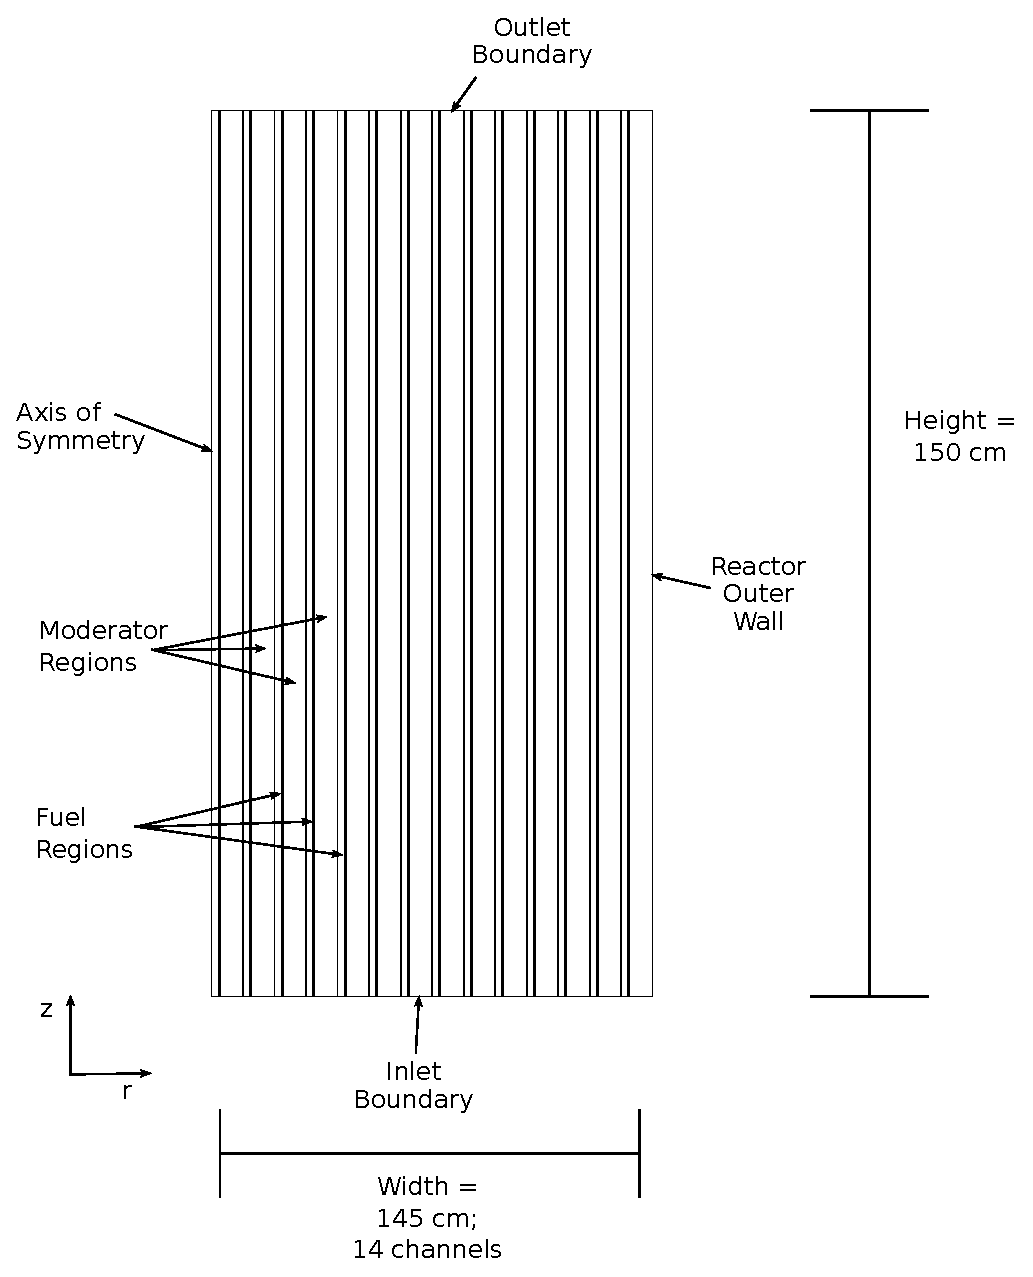
\includegraphics{geometry.eps}
  \label{fig:geom}
  \caption{A sketch of the \gls{MSR} model geometry}
\end{figure}


The model fuel composition is the \gls{BOL} enriched uranium composition in the 
\gls{MSRE} and is given in \Cref{table:comp} \cite{robertson_msre_1965}.


\begin{table}[htpb]
  \begin{center}
    \begin{tabular}{l | r}
      Component & Mass Fraction\\\hline\hline
      Li-7 & .1090\\
      Li-6 & 5$\times$10$^{-6}$\\
      F-19 & .6680\\
      Be-9 & .0627\\
      U-235 & .0167\\
      U-238 & .0344\\
    \end{tabular}
  \end{center}
        \caption{Fuel salt composition is the \gls{BOL} enriched
        uranium composition in the \gls{MSRE} design
        \cite{robertson_msre_1965}.}
  \label{table:comp}
\end{table}

Other simulation inputs are outlined in \Cref{table:params}.
We chose a reactor simulation height of 151.75 cm to produce an
approximately critical reactor configuration corresponding to \gls{BOL}
\gls{MSRE} composition. This differs from the actual \gls{MSRE} height, which 
was 162.56 cm.

\begin{table}[htpb]
  \begin{center}
    \begin{tabular}{l|c|c|c}
      Parameter & Value & Units & Source\\\hline\hline
      Inlet temp. & 922 & $K$ & \gls{MSRE} nominal \cite{robertson_msre_1965}\\
      Wall temp. & 922 & $K$ & \gls{MSRE} nominal \cite{robertson_msre_1965}\\
      Neutron groups & 2 & 1 & User\\
      Precursor groups & 6 & 1 & User\\
      Reactor radius & 72.5 & $cm$ & $\approx$\gls{MSRE} radius (70.2 cm) \cite{robertson_msre_1965}\\
      Reactor height & 151.75 & $cm$ & User\\
      $k{_f}$ & .0553 & $W cm^{-1} K^{-1}$ & \cite{robertson_msre_1965}\\
      $c_{p,f}$ & 1967 & $J K^{-1} kg^{-1}$ & \cite{robertson_msre_1965}\\
      $\rho_f$ & $2.146\cdot 10^{-3} e^{-\alpha_f (T_f - 922)}$ & $kg\ cm^{-3}$ & \cite{robertson_msre_1965}\\
      $\alpha_f$ & $2.12\cdot 10^{-4}$ & $K^{-1}$ &
      \cite{haubenreich_experience_1970}\\
      $k_g$ & .312 & $W cm^{-1} K^{-1}$ & \cite{cammi_multi-physics_2011}\\
      $c_{p,g}$ & 1760 & $J K^{-1} kg^{-1}$ & \cite{cammi_multi-physics_2011}\\
      $\rho_g$ & $1.86\cdot 10^{-3} e^{-\alpha_g (T_g - 922)}$ & $kg\ m^{-3}$ &
      \cite{robertson_msre_1965}\\
      $\alpha_g$ & $1.8\cdot 10^{-5}$ & $K^{-1}$ &
      \cite{haubenreich_experience_1970}\\
    \end{tabular}
  \end{center}
  \caption{Simulation input parameters}
  \label{table:params}
\end{table}


\section{Results \& Discussion}

Group fluxes are shown in \Cref{fig:group1,fig:group2}. The cosinusoidal shapes 
in radial and
axial directions are caused by the vacuum boundary conditions. Both the fast and thermal fluxes are striated, with
the fast group preferring the fuel and the thermal group preferring the moderator.

\begin{figure}[htpb]
  \centering
  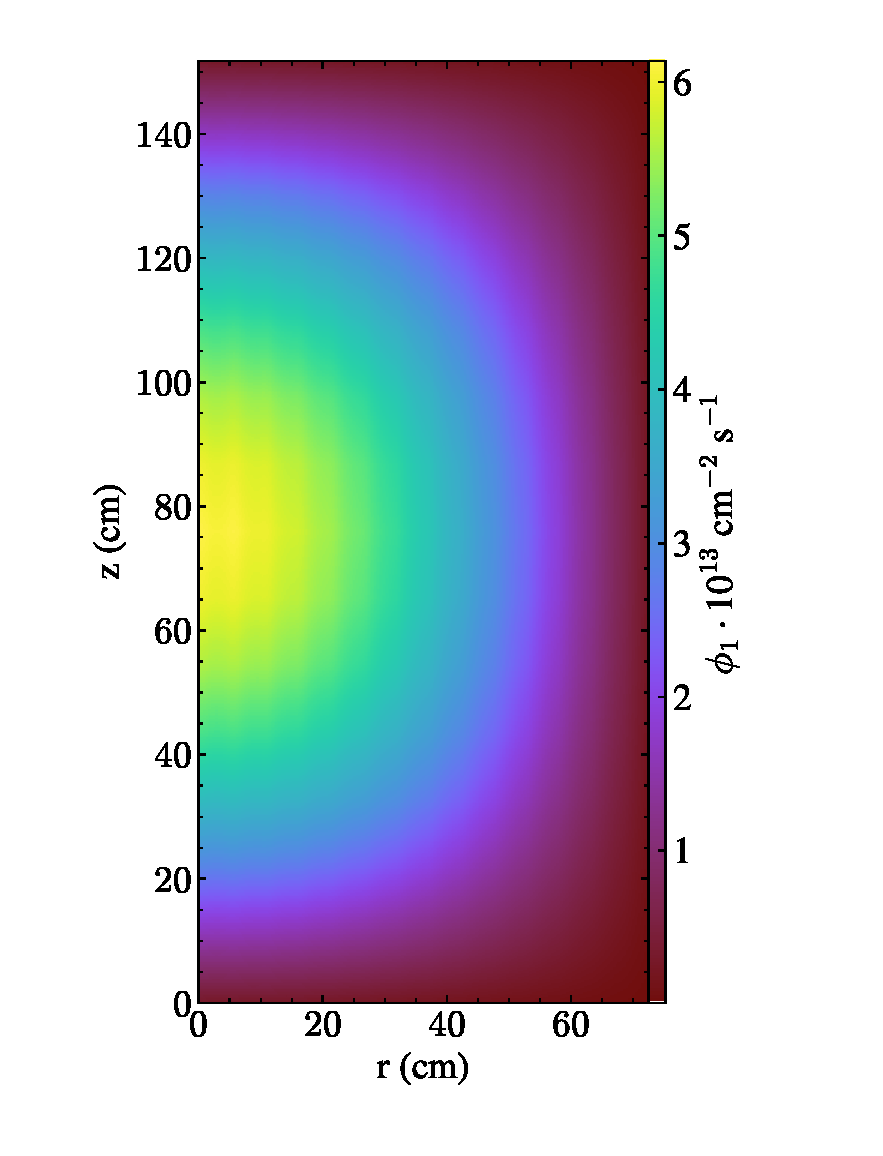
\includegraphics{2d_gamma_heating_group1.eps}
        \caption{The group 1 flux in this 2-D cylindrical axisymmetric model
        has the anticipated magnitude and canonical cosine shape ($r=0$ is center of core). }
  \label{fig:group1}
\end{figure}

\begin{figure}[htpb]
  \centering
  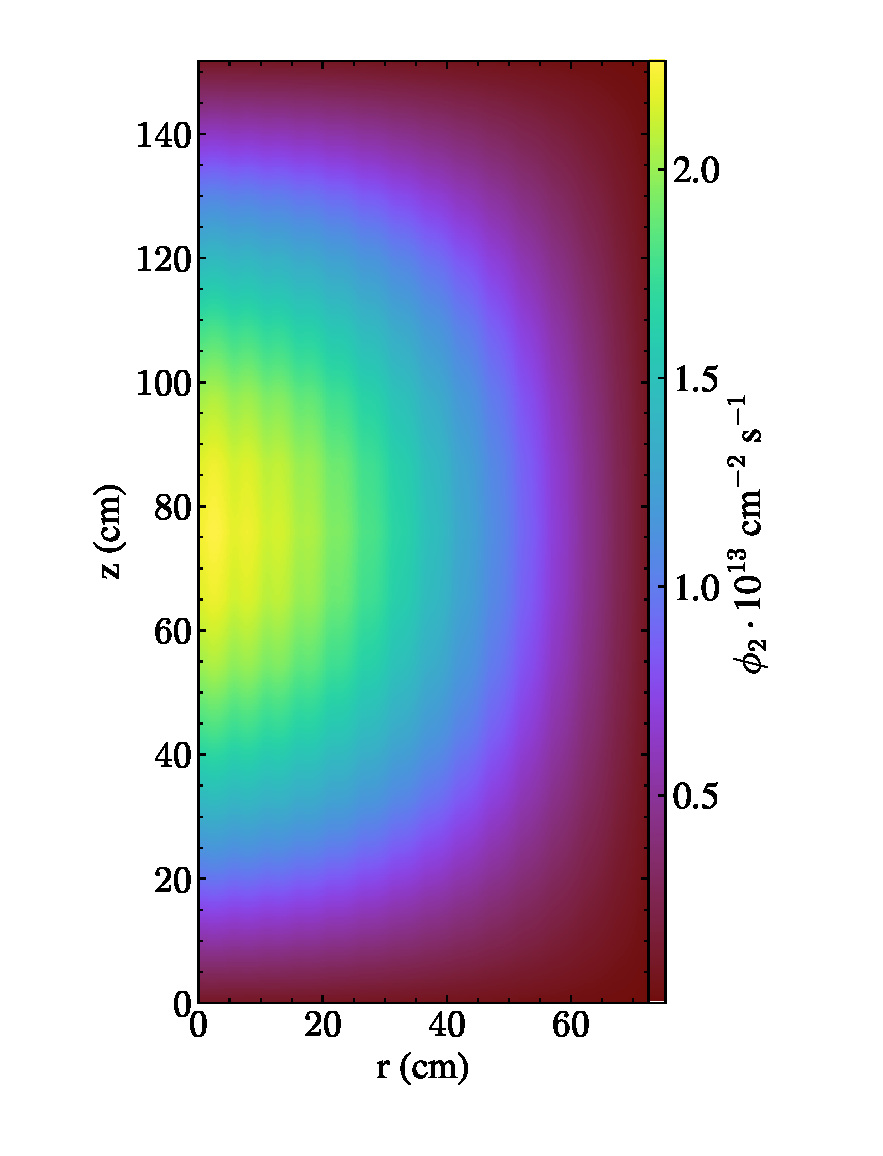
\includegraphics{2d_gamma_heating_group2.eps}
        \caption{The group 2 flux in this 2-D cylindrical axisymmetric model
        has the anticipated magnitude and canonical cosine shape ($r=0$ is center of core). }
  \label{fig:group2}
\end{figure}

In \Cref{fig:temp} the temperature rises along the reactor height because of 
fuel advection. The temperature gradient is negative in the 
radial direction, as expected.

\begin{figure}[htpb]
  \centering
  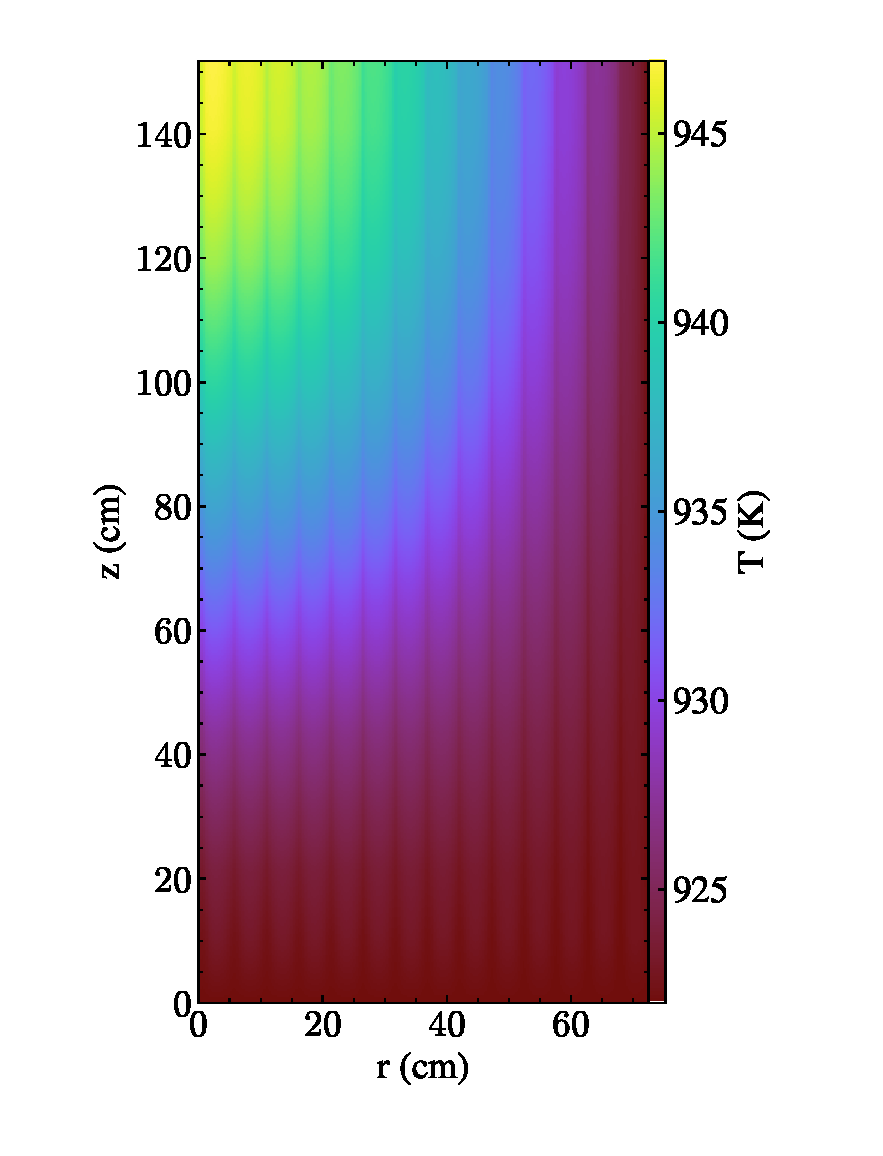
\includegraphics{2d_gamma_heating_temp.eps}
        \caption{The reactor core temperature peaks near the reactor outlet in
          this 2-D axisymmetric model because of fuel advection ($r=0$ is center
          of core). Because of heating by gammas and other radiation the
          moderator regions are hotter than the fuel, consistent with
          observations of the \gls{MSRE}}
  \label{fig:temp}
\end{figure}

\Cref{fig:pre1} shows the concentration of the longest lived precursor in the
reactor. Not surprisingly, the channel concentrations are higher in fuel channels
with higher neutron fluxes and corresponding fission
events. Because of the small decay constant of the precursor, the maximum
concentration in any given channel occurs at the core outlet due to advection.

\begin{figure}[htpb]
  \centering
  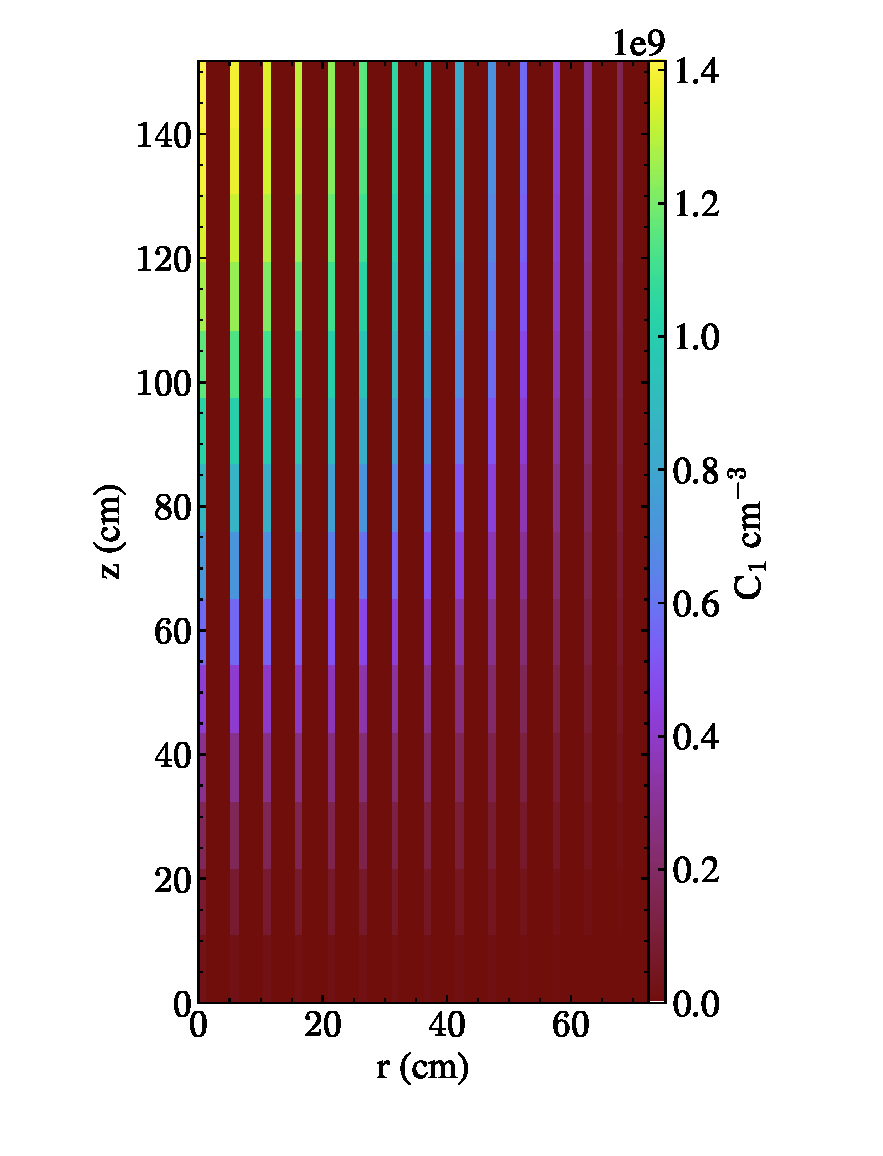
\includegraphics{2d_gamma_heating_pre1_scaled.eps}
        \caption{The concentration of the group of longest lived precursors
        ($\lambda = 1.24\cdot 10^{-2} s^{-1}$) peaks near the reactor outlet
        in this 2-D axisymmetric model ($r=0$ is center of core).}
  \label{fig:pre1}
\end{figure}

With its much larger decay constant, the sixth and last precursor has its
maximum concentration around the center-plane of the reactor as shown in
\Cref{fig:pre6}. As for all other precursors, its concentration decreases with
increasing radius and decreasing neutron flux.

\begin{figure}[htpb]
  \centering
  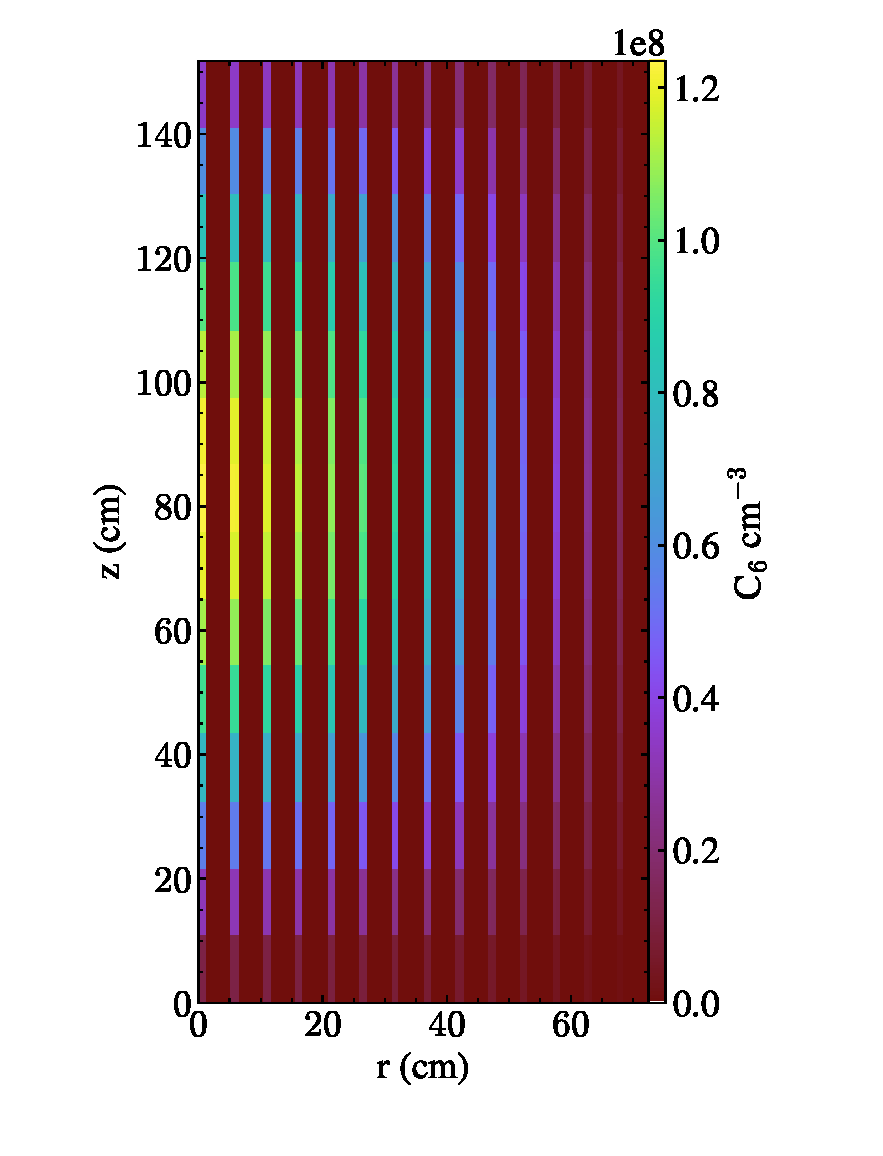
\includegraphics{2d_gamma_heating_pre6_scaled.eps}
        \caption{The concentration of the group of shortest lived precursors
        ($\lambda = 3.07 s^{-1}$) peaks near the reactor center
        in this 2-D axisymmetric model ($r=0$ is center of core).}
  \label{fig:pre6}
\end{figure}

\subsection{Three dimensional simulation capability}

\Cref{fig:3d_group1,fig:3d_temp} show Moltres physics applied to a three
dimensional geometry. The fast group flux (\cref{fig:3d_group1}) is in good
qualitative agreement with the two dimensional axisymmetric case shown in
\cref{fig:group1}. \Cref{fig:3d_temp} is in similarly good agreement with
\cref{fig:temp}. \Cref{fig:3d_temp_fuel_outlet} shows the temperature profile at
the outlet of the reactor (z = H). This three dimensional case contained
1,155,045 degrees of freedom and took only 2.5 hours to solve on 160 Blue Waters
cores.

\begin{figure}[htpb]
  \centering
  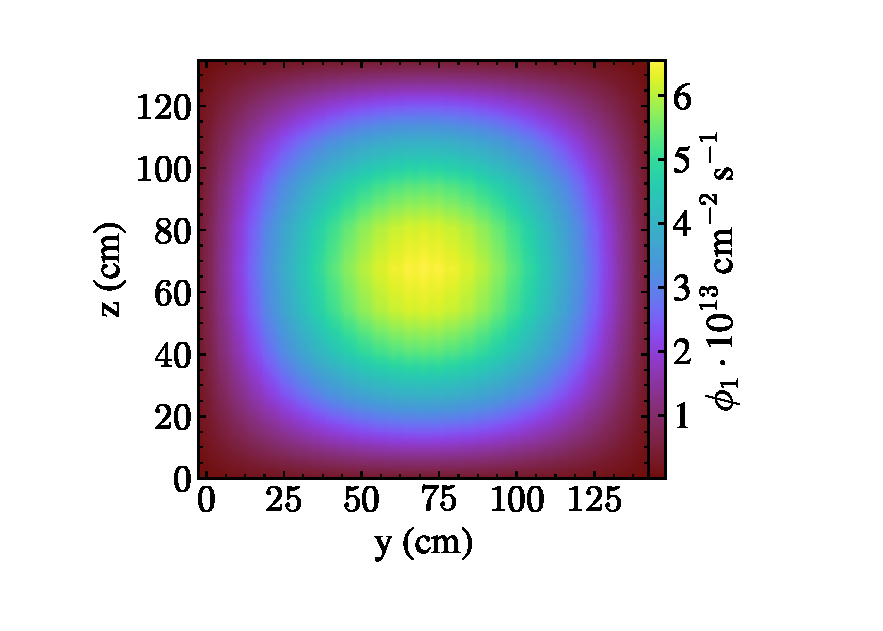
\includegraphics{3d_gamma_heating_group1.eps}
        \caption{Fast flux for 3D \gls{MSRE}-like model. Magnitude and shape in
          good agreement with 2D axisymmetric model (see \cref{fig:group1})}
  \label{fig:3d_group1}
\end{figure}

\begin{figure}[htpb]
  \centering
  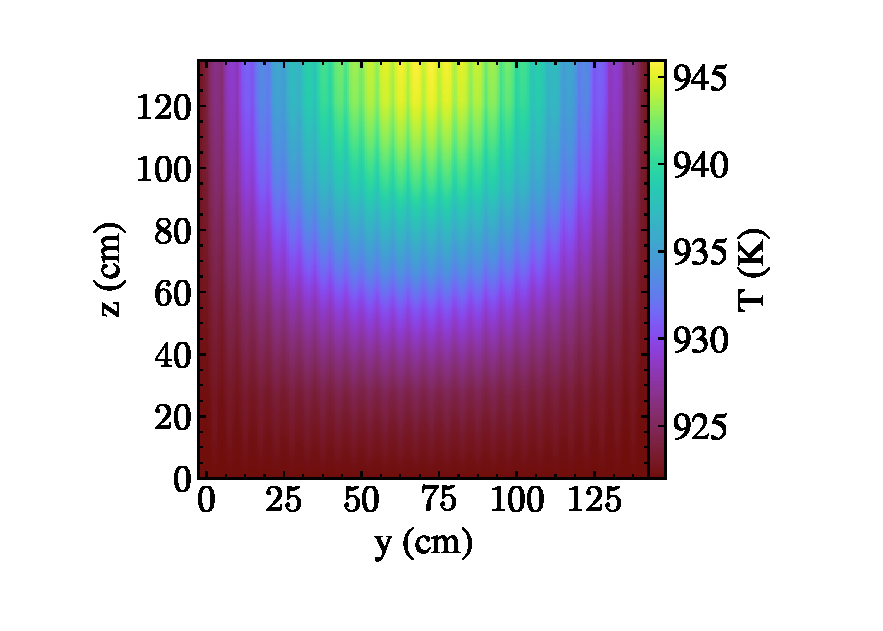
\includegraphics{3d_gamma_heating_temp.eps}
        \caption{Temperature for 3D \gls{MSRE}-like model. Magnitude and shape in
          good agreement with 2D axisymmetric model (see \cref{fig:temp})}
  \label{fig:3d_temp}
\end{figure}

\begin{figure}[htpb]
  \centering
  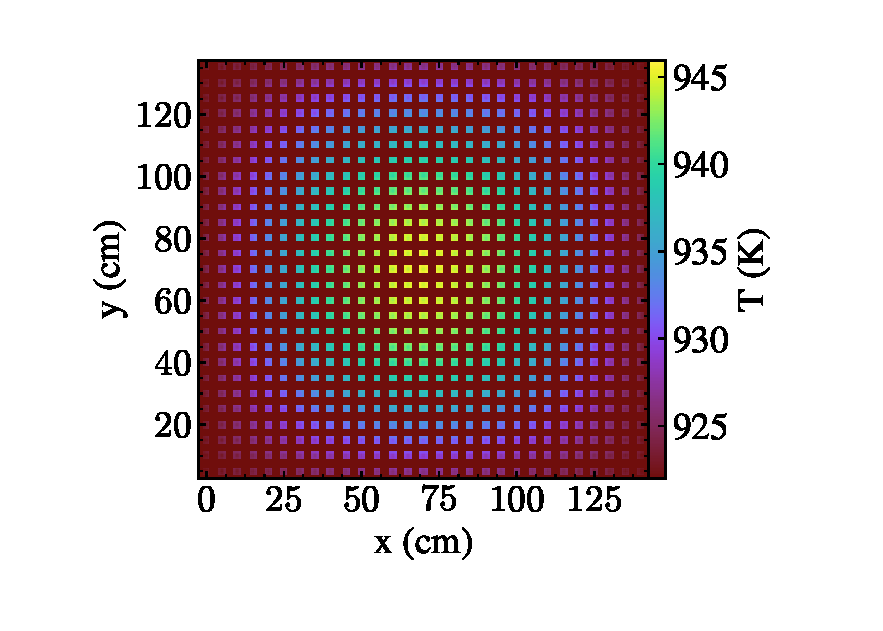
\includegraphics{3d_gamma_heating_z_slice_temp.eps}
        \caption{Temperature at the reactor outlet for 3D \gls{MSRE}-like
          model.}
  \label{fig:3d_temp_fuel_outlet}
\end{figure}



\subsection{Comparison with \gls{MSRE}}

\Cref{fig:temp_compare} shows a comparison between Moltres predicted temperature
profiles with cosinusoidal gamma heating and \gls{MSRE} design models
\cite{briggs_molten-salt_1964} in the hottest channel and adjacent graphite. The
profile shapes are in decent qualitative agreement with both Moltres and
\gls{MSRE} calculations showing a peak in graphite temperature before the
reactor outlet. Fuel temperature increases monotonically in both Moltres and
\gls{MSRE} models. In the \gls{MSRE} design, the moderator
temperature at the reactor inlet is about 20 degrees Fahrenheit larger than the
fuel temperature, whereas the temperatures are about the same in the Moltres
model. This difference is likely because the \gls{MSRE} design model 
neglected axial heat conduction \cite[p. 99]{briggs_molten-salt_1964}.

\begin{figure}[htpb]
    \centering
    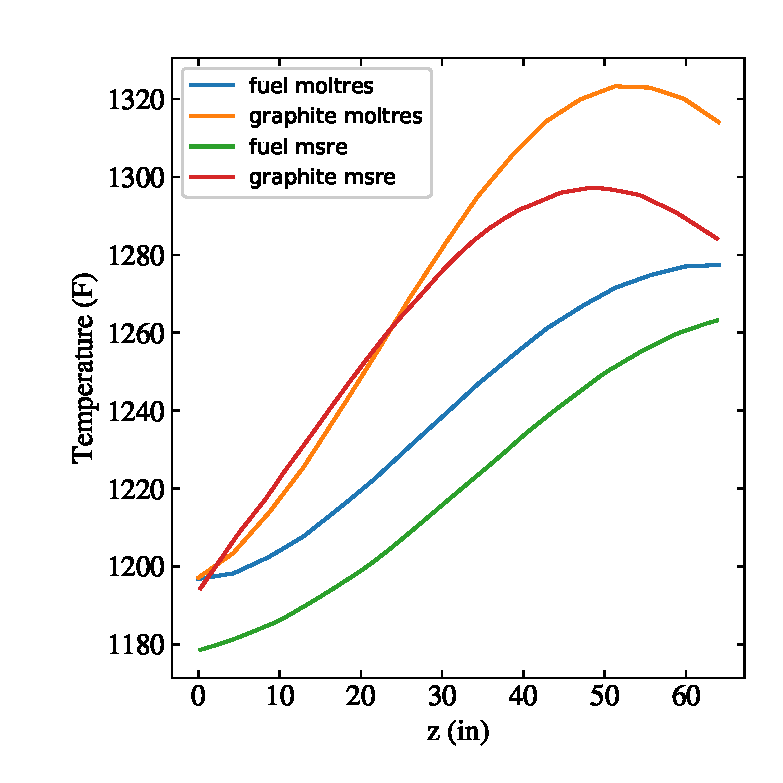
\includegraphics[width=\maxwidth{\textwidth}]{combined_msre_moltres_axial_temps.eps}
    \caption{Moltres and \gls{MSRE} design
      \cite[p. 99]{briggs_molten-salt_1964} predicted axial temperature profiles in hottest channel
      and adjacent graphite}
    \label{fig:temp_compare}
\end{figure}


\Cref{fig:radial_fluxes_compare} compares the fast and thermal neutron fluxes at
the reactor mid-plane ($z=H/2$) for Moltres and \gls{MSRE} design models. Local
thermal flux growth and fast flux decay in moderator regions and visa versa in
fuel regions are apparent in the Moltres calculation. The Moltres flux
magnitudes are in good agreement with the magnitudes from the \gls{MSRE} design
calculations \cite[p. 92]{briggs_molten-salt_1964}. The peak fast to thermal
flux ratio is approximately 3.5 in the \gls{MSRE} design calculation as opposed
to a ratio of 3 for the Moltres calculation. Control rod thimbles and an extra
volume of surrounding fuel not included in the Moltres calculations cause the
depression in the thermal flux in the \gls{MSRE} profile.

\begin{figure}[htpb]
    \centering
      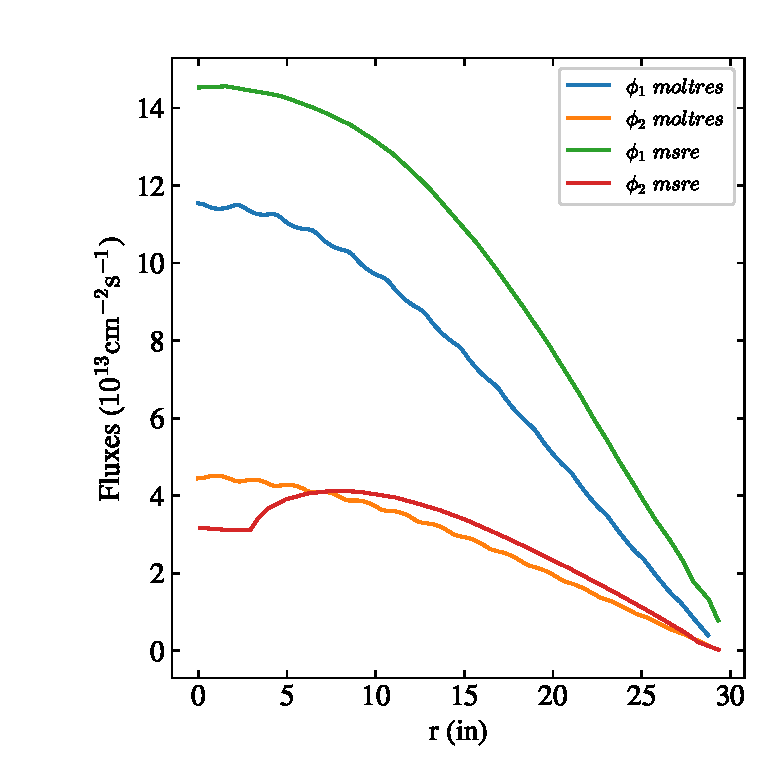
\includegraphics[width=\maxwidth{\textwidth}]{combined_msre_moltres_radial.eps}
      \caption{The thermal and fast flux profiles at the core mid-plane
        ($z=H/2$) for the Moltres 2-D cylindrical axisymmetric model and the
        \gls{MSRE} design model \cite[p. 92]{briggs_molten-salt_1964} ($r=0$ is
        radial center of core).}
    \label{fig:radial_fluxes_compare}
\end{figure}

\Cref{fig:axial_fluxes_compare} compares the axial flux profiles calculated by
Moltres and the \gls{ORNL} \gls{MSRE} design model. The radii for the plots are
chosen to correspond to the peak of the thermal flux in both cases; for the
\gls{ORNL} calculations this is 8.4 inches from the core center-line because of
the effect of the control rod thimbles and extra fuel along the
center-line. Once again, the plots are in decent agreement. The \gls{ORNL}
calculations include the lower and upper plena which are not included in this
report's Moltres model. Consequently, the \gls{MSRE} lines extend to lower and
higher z-values than the Moltres lines. Additionally, absorption
in the plena cause deviation of the thermal flux from a sinusoidal shape in the
\gls{MSRE} design case.

\begin{figure}[htpb]
    \centering
    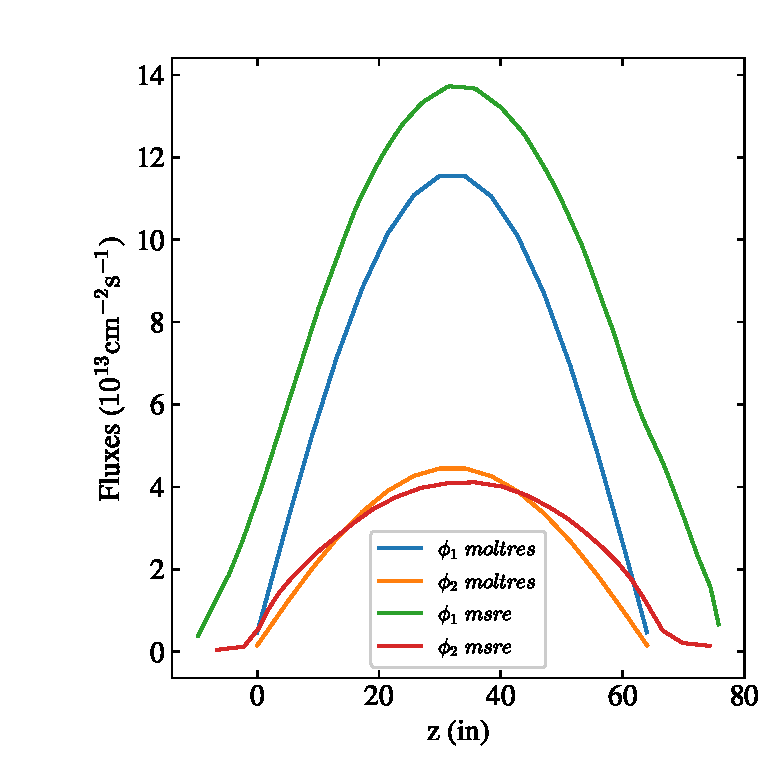
\includegraphics[width=\maxwidth{\textwidth}]{combined_msre_moltres_axial.eps}
    \caption{Moltres axial flux profiles along core center line and \gls{MSRE}
      design axial flux profiles 8.4 inches from core center line \cite[p. 91]{briggs_molten-salt_1964}.}
    \label{fig:axial_fluxes_compare}
\end{figure}

\subsection{Scaling study}

As described earlier, Moltres runs naturally in parallel. To test its
performance, we conducted a scaling study with a typical 2D axisymmetric input
file. \Cref{fig:scaling_study} shows Moltres' performance. The solution
time follows the ideal closely; slight deviations are expected due to
the expense of communication and the nature of iterative solvers. More
parallelism means the solution process uses more ``older'' information, 
which leads to slower convergence in terms of iterations 
\cite{satish_balay_petsc_2015}.

\begin{figure}[htpb]
  \centering
  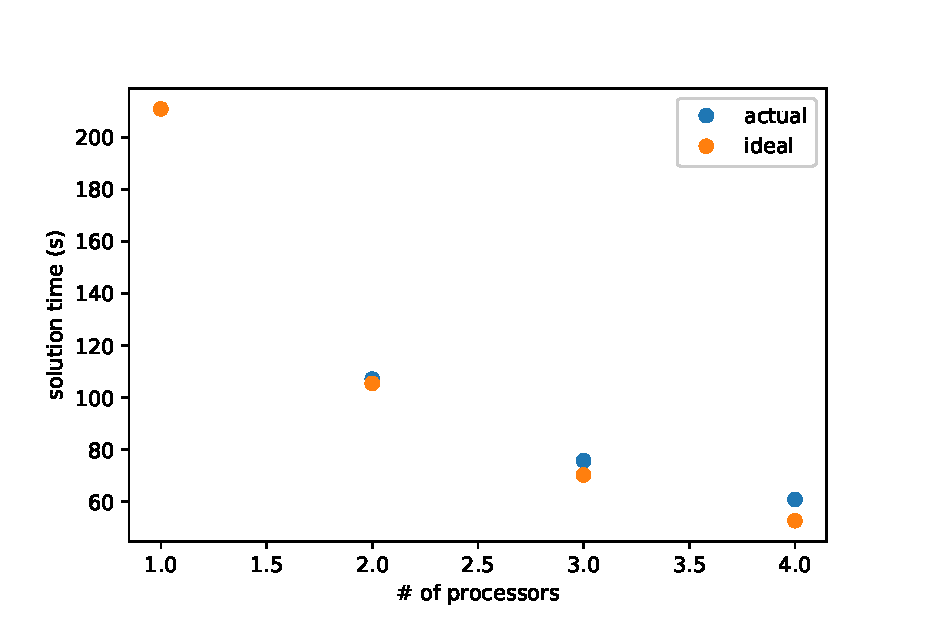
\includegraphics{scaling_study.eps}
  \caption{Moltres performance on a typical 2D axisymmetric problem for
    different numbers of processors}
  \label{fig:scaling_study}
\end{figure}


\section{Conclusion}

This work introduces the open source \gls{MSR} simulation code Moltres. Moltres
solves arbitrary-group neutron diffusion, temperature, and precursor governing
equations in anywhere from one to three dimensions and can be deployed on an
arbitrary number of processing units. The 2D-axisymmetric and 3D models
presented here employ heterogeneous group constants for fuel and moderator
regions generated with SCALE. Fuel volume fraction and fuel salt composition are
based on the \gls{MSRE}. Neutron fluxes show expected cosinusoidal shapes in
radial and axial directions with visible striations between fuel and moderator
regions. The fast group flux is enhanced in fuel regions while the thermal group
flux in enhanced in moderator regions. Due to advection the temperature profile
in the fuel increases monotonically in the direction of salt flow, while the
moderator temperature exhibits a maximum between the mid-plane and outlet. The
role of advection is also seen in precursor concentrations. Long lived
precursors exhibit maximum concentrations at the core outlet. As the decay
constant increases across precursor groups the maximum concentrations moves
towards the reactor center where the precursor production rate is
maximum. Results from 2D-axisymmetric and 3D models show good qualitative
agreement. Moreover, Moltres results compare favorably with the actual design
calculations of the \gls{MSRE}. Moltres demonstrated strong parallel scaling on a
typical model problem. Future Moltres publications will highlight
transient simulation cases investigating control rod ejection, single channel
blockage, loss of flow, and loss of secondary cooling.

\FloatBarrier

\section{Acknowledgments}

All figures in this paper were generated using the python package yt
\cite{turk_yt:_2011}. The package engauge-digitizer
\cite{mark_mitchell_markummitchell/engauge-digitizer:_2017} was used to convert
rasterized \gls{MSRE} line plots into point data for plotting alongside Moltres
data.

This work was supported by the University of Illinois Department of Nuclear, 
Plasma, and Radiological Engineering, the National Center for Supercomputing 
Applications, and the University of Illinois Blue Waters Professors program. 
Undergraduate researcher Gavin Ridley was supported through NSF REU Site award 
1659702, ``INCLUSION - Incubating a New Community of Leaders Using Software, 
Inclusion, Innovation, Interdisciplinary and OpeN-Science.''

Finally, the authors would like to thank Matthew Turk and the Data Exploration 
Lab for co-supporting Dr. Lindsay during his postdoctoral appointment.

\clearpage
\printglossary[type=\acronymtype]
\bibliographystyle{unsrt}
\bibliography{Moltres}
\end{document}
